%
% Mensch vs. Maschiene
% Abschlussarbeit (Bachelor)
%
% Thema: Erstellung einer Browser Extension zur Usability Evaluierung von beliebigen Web-Applikationen über Heatmaps.
% Betreuer 1: Prof. Dr. Targo Pavlista
% Betreuer 2: Siamak Haschemi
%
% @author Christian Bromann <contact@christian-bromann.com>
%

\section{Mensch vs. Maschine}

Zu Beginn dieses Kapitels wurde Usability als eine Art Bestreben nach ergonomischer Software definiert. In dem Mensch-Maschinen-System spielte dabei der User eine wichtige Schlüsselkomponente zum Erreichen dieses Vorhabens. Je nach Alter, Erfahrung und Intention nutzen Menschen eine Software sehr unterschiedlich. Dadurch scheint es, als ob immer eine Person zur Bestimmung der Usability involviert sein muss, um ein aussagekräftiges Resultat zu erzielen. Es stellt sich die Frage auf, ob dem wirklich so ist?\\
\\
Der Begriff \textit{Informatik} ist die Komposition aus den Wörtern Information und Automatik / Mathematik. Jeder Informatiker strebt danach, für doppelt ausgeführte Handlungen einen Automatismus zu entwerfen, um sich unnötige Arbeit zu sparen. Dies soll jedoch nicht suggerieren, dass Informatiker faule Menschen sind \cite{lazy}. Beim Usability-Engineering findet ebenfalls ein immer wieder auftretender Prozess der Analyse und Verbesserung statt. Dieser ist meist immer mit hohen Kosten und Zeitaufwänden verbunden. Zudem führen Usability-Tests aufgrund des sogenannten \textit{\glqq Evaluator Effect\grqq{}} \cite{anzahlTestpersonen} nicht immer zu den gewünschten Ergebnissen. Ein Grund dafür ist die kritische Rolle der Gutachter. Studien haben bewiesen, dass diese zu unterschiedlichen und teilweise falschen Interpretationen neigen und Probleme beweisen, die bereits entdeckt wurden.\\
\\
Nicht nur aufgrund dieser Tatsachen haben sich bereits viele Usabiliy Experten mit der Frage beschäftigt, wie die Benutzerfreundlichkeit auf Webseiten automatisiert getestet und in Ergebnisse überführt werden kann \cite{automatisierteUsabilityTests}. Daraus entstanden im Laufe der Zeit verschiedene Prototypen, die sich bereits auf dem Markt etablieren konnten. Diese nutzen entweder die bisher entwickelten Normen der Organisationen für Standardisierung oder versuchen ein mögliches Nutzerverhalten vorauszusehen. Letztere Herangehensweise wurde bereits von vielen Wissenschaftlern kritisiert, da die dafür verwendeten Algorithmen zum Vorhersagen des Verhaltens zu teilweise beirrenden Ergebnissen führen.\\
\\
Anders dagegen nutzt das Framework \textit{USEFul} ein Regelset, welches den verschiedenen Normen der Usability entspricht, zur Analyse der Seite und zur Einschätzung der Benutzerfreundlichkeit. Dieses Regelset wird dabei in drei verschiedene Kategorien untergliedert. Eine Kategorie entspricht den Richtlinien, die das Tool im vollem Umfang evaluieren und kontrollieren kann. Sie sind ablesbar und über Parameter klassifizierbar. Die nächste Kategorie beinhaltet Normen, die nur teilweise erfassbar und messbar sind. Zu abstrakte Usability-Regeln fallen schließlich in die letzte Kategorie. Diese sollten von den Evaluatoren manuell kontrolliert werden, ob sie für die aktuell getestete Seite zutreffen oder nicht. Zusätzlich werden die Regeln von 1 bis 5 priorisiert, um wichtigen Guidelines eine höhere Gewichtung zu geben.\\
\\
Laut Nielsen ist die URL ein Teil des User Interfaces und bestimmt somit ebenfalls die Usability einer Webseite \cite{urlasui}. Sie sollte so kurz und prägnant wie nötig gehalten werden und sich an der Seitenstruktur orientieren. Diese nicht ganz unwichtige Regel ist ein gutes Beispiel, um aufzuzeigen, wie USEFull eine Website automatisiert evaluieren kann. Nachdem sich das Tool die Source Dateien der Seite gezogen hat, sucht es nach allen Link Tags auf der Seite. Diese Tags beinhalten die Ziel URL im \textit{href} Attribut. Überschreitet die URL die Länge der vorher festgelegten maximalen Anzahl von Zeichen, so verstößt die Seite gegen diese Regel. Berechnet man nun das Verhältnis der korrekten gegenüber der zu langen URLs, so erhält man sogar eine Qualitätsrate, die zwischen verschiedenen Tests verglichen werden kann. Abbildung \ref{usefull} zeigt die letztendliche Gesamtauswertung des Frameworks. Die Ergebnisse werden innerhalb der jeweiligen Kategorien aufgelistet, nach Priorität sortiert und erklärt.

\vspace{0.3cm}
\begin{center}
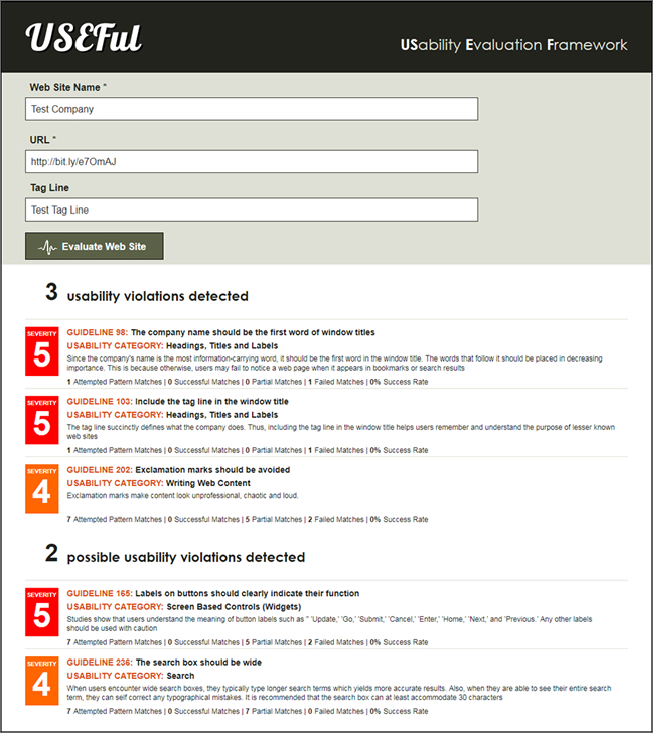
\includegraphics[scale=1]{./images/usefull}
\end{center}
\begin{figure}[htb]
   \centering
   \caption{Ansicht einer automatisierten Auswertung des USEFull Frameworks\\\textbf{Quelle:} http://usabilitygeek.com/wp-content/uploads/2012/03/USEFul-A-Framework-To-Automate-Website-Usability-Evaluation-Analysis.jpg}
    \label{usefull}
\end{figure}

Unglücklicherweise ist der Prototyp noch nicht für die Öffentlichkeit zugänglich. Lediglich Papers und Usability-Blogs beschreiben die Funktionsweise und Features des Tools. Nichtsdestotrotz scheint der Traum nach einer komplett automatisierten Usability-Evaluierung auch damit nicht erfüllt zu sein. Da nicht wirklich alle Regeln mit Algorithmen überprüft werden können, bleibt es letztendlich die Aufgabe eines Experten zu entscheiden, ob die Ergebnisse der Auswertung repräsentativ genug sind, um die Qualität der Usability richtig einzustufen. Dennoch können viele Aspekte automatisiert kontrolliert werden und dadurch bei der Entwicklung frühzeitig die Probleme aufdecken, die ohne das Tool erst durch teure Tests erkannt werden.